A continuación se describe el producto obtenido, siguiendo las diferentes fases de la metodología de trabajo y las herramientas descritas con anterioridad.

\paragraph{Autentificación de un usuario en el sistema: } Solicitud de acceso, utilizando credenciales de acceso los cuales son ingresados por el usuario. Si las credenciales son válidas, se redirecciona a las interfaces de la OE interesada o a la del Administrador (vea \textbf{Figura \ref{fig: Login}}).

\begin{figure}[h]
    \centering
    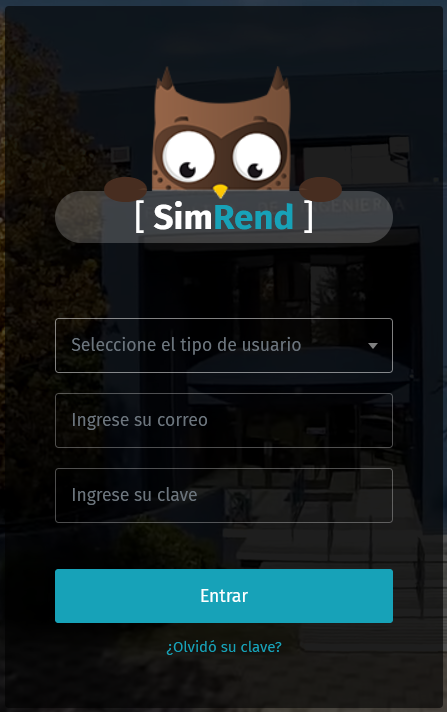
\includegraphics[width=0.3\textwidth]{Imagenes/Login.PNG}
    \caption{\label{fig: Login}Vista de ingreso al sistema.}
\end{figure}

\paragraph{Recuperación de acceso a una cuenta de una OE: } Solicitud de una nueva clave de acceso en caso de que el usuario la olvide ingresando el correo de la OE a la que pertenece. Una vez ingresada esta información se solicita la recuperación de cuenta al servidor, el cual envía un correo con la nueva clave de acceso al usuario (vea \textbf{Figura \ref{fig: RecuperarClave}}).

\begin{figure}[h]
    \centering
    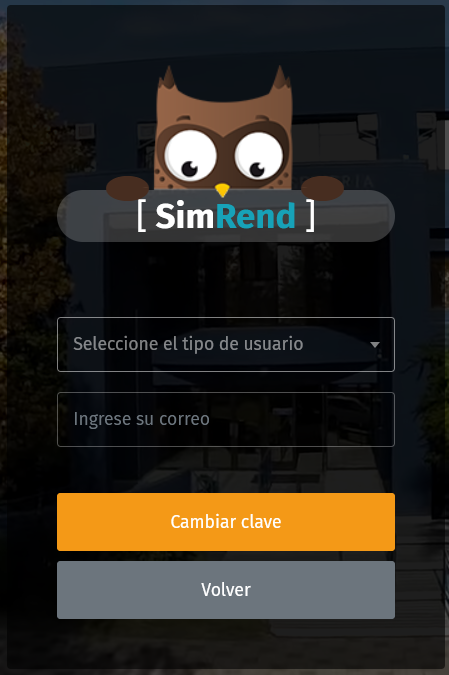
\includegraphics[width=0.4\textwidth]{Imagenes/RecuperarClave.PNG}
    \caption{\label{fig: RecuperarClave}Vista de recuperar clave.}
\end{figure}

\paragraph{Búsqueda de solicitudes: } En esta etapa de la aplicación se encuentran todas las solicitudes realizadas por la OE, en donde el usuario puede visualizar los resúmenes de la solicitudes y tener la opción de ver en detalle cada una de ellas. Además, se encuentra la opción de realizar búsquedas de solicitudes a través del nombre o la fecha del evento (vea \textbf{Figura \ref{fig: Busquedas}}).

\begin{figure}[h]
    \centering
    \includegraphics[width=0.69 \textwidth]{Imagenes/Busqueda.PNG}
    \caption{\label{fig: Busquedas}Vista de búsqueda de solicitudes.}
\end{figure}

\paragraph{Solicitud: }Esta etapa consta de 4 fases las cuales ayudan a la confección de la solicitud a presentar a la Dirección correspondiente de cada OE. Estas fases se detallan a continuación. 

    \subparagraph{\emph{Datos principales de la Solicitud: }} Formulario que solicita el nombre, fecha de inicio, fecha de término, lugar y monto del evento, el responsable a cargo de la solicitud y la cantidad de participantes, la cual puede ser para un grupo de personas específico o masivo (e indeterminado), según sea el caso (vea \textbf{Figura \ref{fig: DatosPrincipales}}).

    \begin{figure}[h]
        \centering
        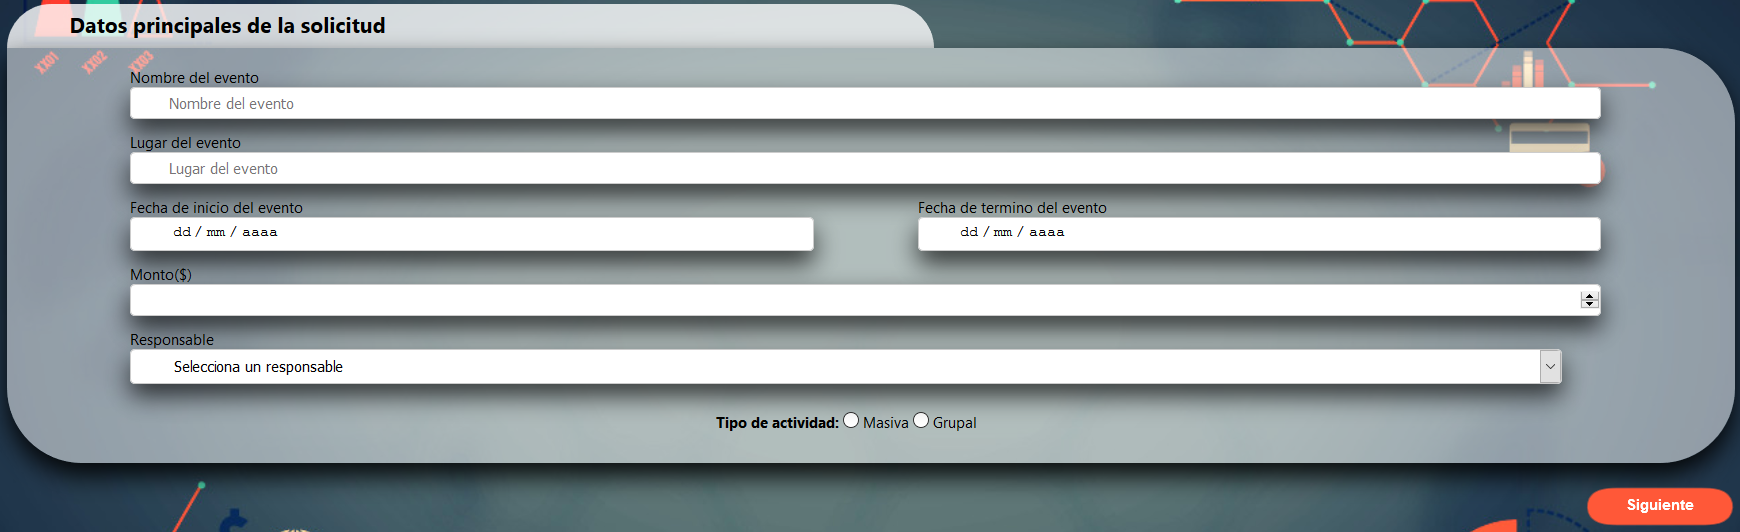
\includegraphics[width= 0.8\textwidth]{Imagenes/DatosPrincipales.PNG}
        \caption{\label{fig: DatosPrincipales}Vista que obtiene los datos principales de una Solicitud.}
    \end{figure}

    \subparagraph{\emph{Categoría: }} En esta etapa se solicitan todas las categoría de los gastos que se realizan dentro del evento para el cual se está realizando la solicitud (vea \textbf{Figura \ref{fig: Categorias}}).

    \begin{figure}[h]
        \centering
        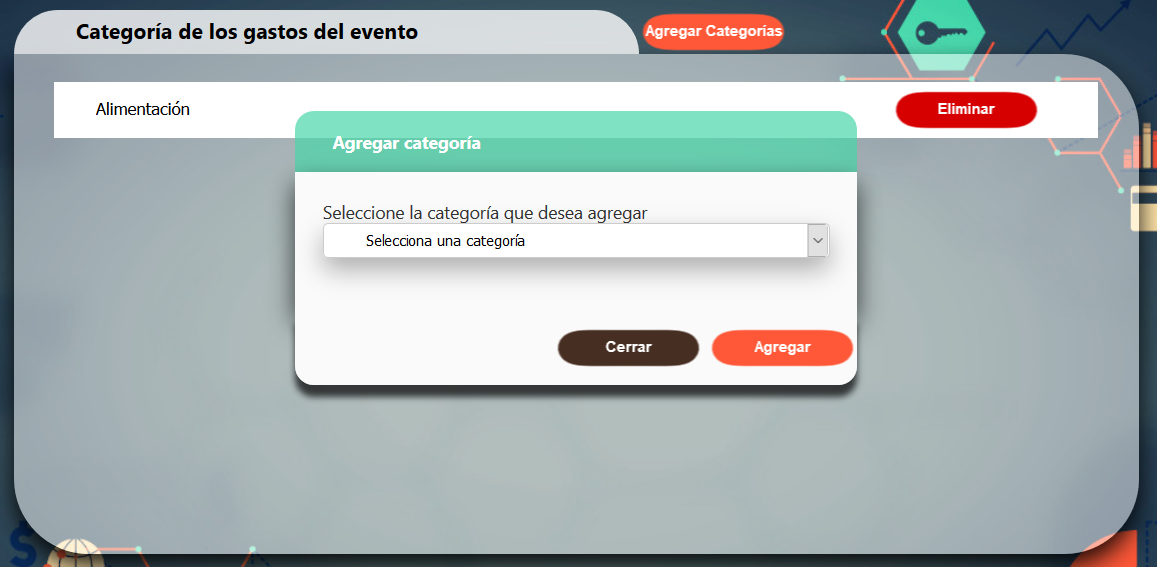
\includegraphics[width= 0.69\textwidth]{Imagenes/Categoria.PNG}
        \caption{\label{fig: Categorias}Vista que obtiene las categorías en que incurren los gastos.}
    \end{figure}

    \subparagraph{\emph{Participante: }} Formulario que solicita el nombre y RUT de los participantes de la actividad. Esta vista sólo se visualiza si en la etapa de \textbf{Datos principales de la solicitud} se indica que es para un grupo de personas específico (vea \textbf{Figura \ref{fig: Personas}}). 

    \begin{figure}[h]
        \centering
        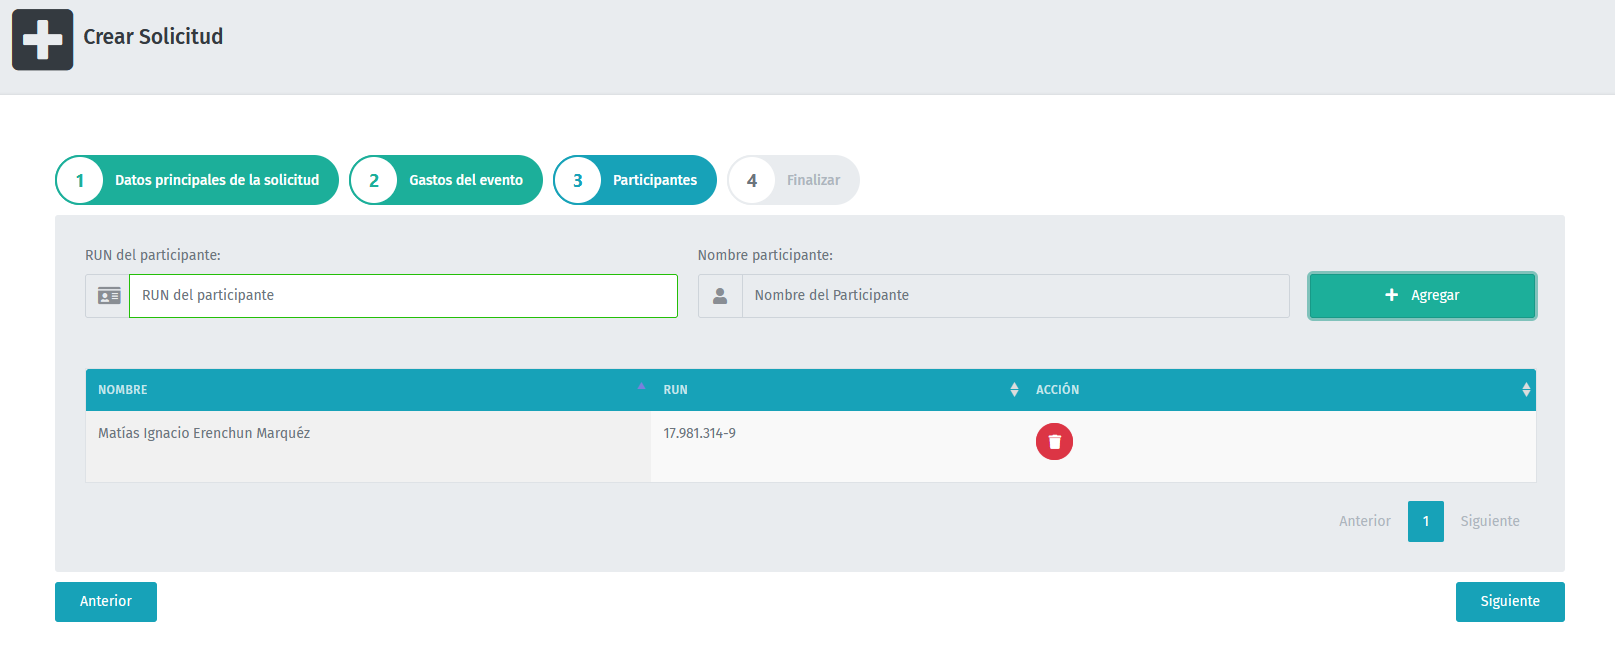
\includegraphics[width= 0.8\textwidth]{Imagenes/AgregarPersonas.PNG}
        \caption{\label{fig: Personas}Vista que obtiene los datos de los participantes del evento.}
    \end{figure}

    \subparagraph{\emph{Resumen: }} Etapa que muestra los datos principales de la solicitud y a su vez da la opción de generar el PDF de la solicitud (vea \textbf{Figura \ref{fig: ResumenSolicitud}}).

    \begin{figure}[h]
        \centering
        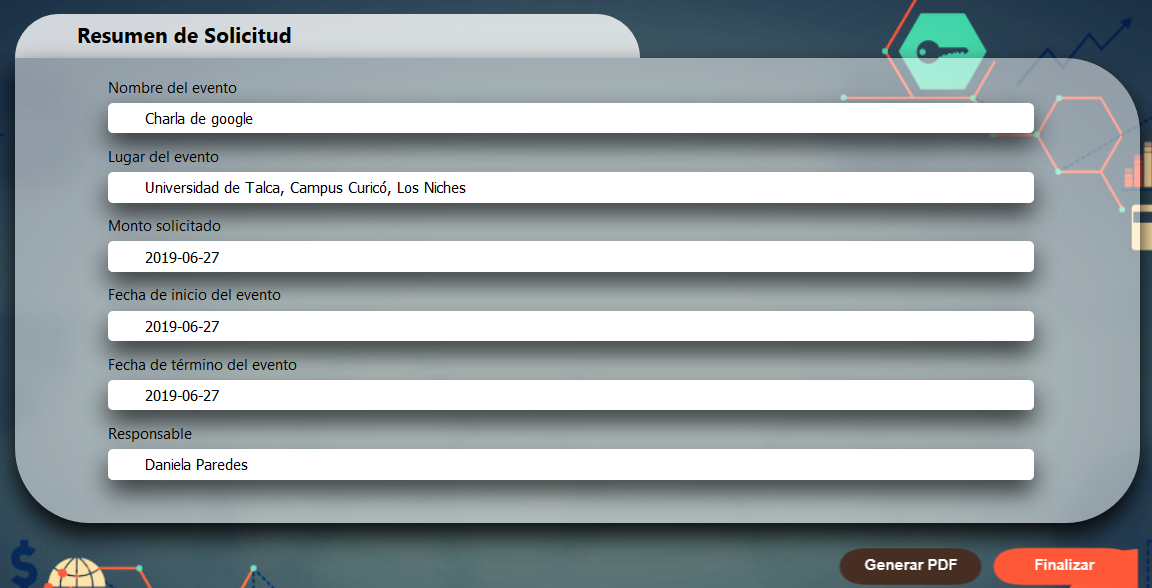
\includegraphics[width= 0.8\textwidth]{Imagenes/Resumen.PNG}
        \caption{\label{fig: ResumenSolicitud}Vista que muestra el resumen de los datos ingresados para la solicitud.}
    \end{figure}

\paragraph{Resolución: } En esta etapa se acepta o rechaza la solicitud. En caso de ser aceptada se procede a ingresar los datos principales de la RU enviada por la Casa de Estudios a la OE interesada, los cuales son el número de la resolución y el año de creación. Además, se solicita que se adjunte una copia digitalizada y en formato PDF de la RU correspondiente a la aceptación de la Solicitud enviada por la OE (vea \textbf{Figura \ref{fig: Resolucion}}).

\begin{figure}[h]
    \centering
    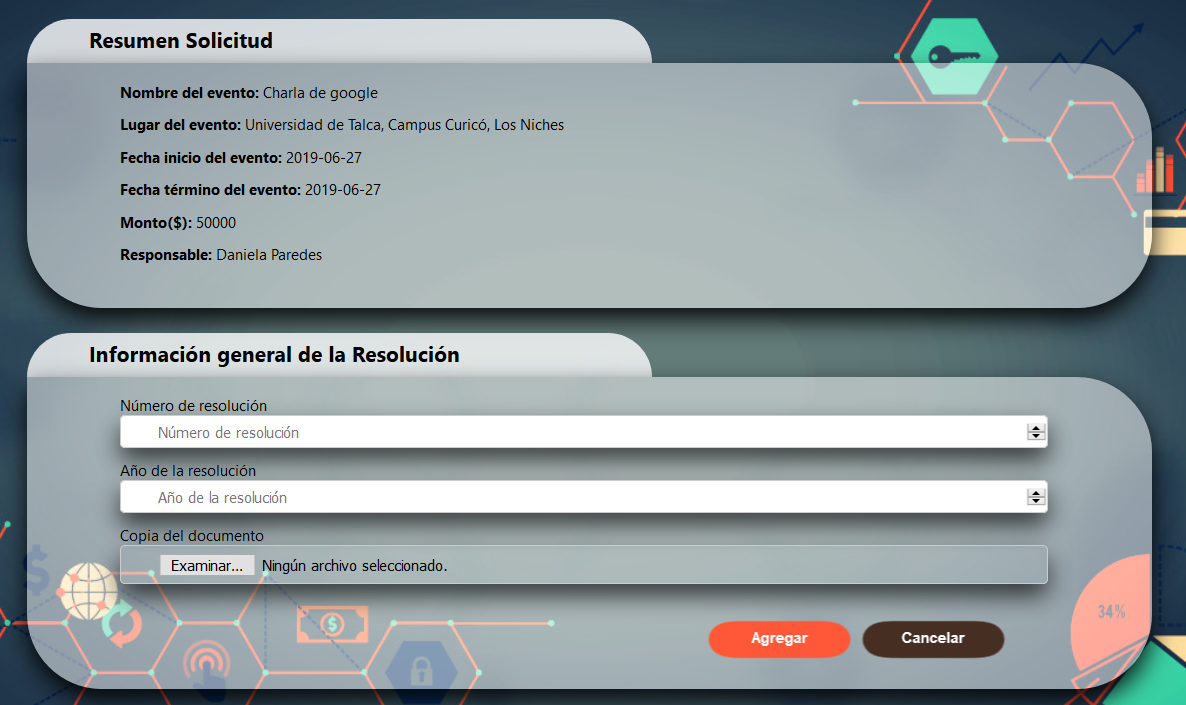
\includegraphics[width= \textwidth]{Imagenes/Resolucion.PNG}
    \caption{\label{fig: Resolucion}Vista que muestra el resumen de los datos ingresados para la solicitud y obtiene los datos principales de la RU.}
\end{figure}

\paragraph{Rendición: } Tras la aceptación de la Solicitud y el ingreso de los datos de la RU que la aprueba, se procede a realizar la Rendición correspondiente al evento. Si bien los datos principales de la Rendición tales como el nombre de la organización, el número de la resolución y el responsable del evento, entre otros, se obtiene automáticamente de los datos registrados en el sistema, el monto total rendido tiene dependencia del registro de documentos (boletas y/o facturas) (vea \textbf{Figura \ref{fig: Rendicion}}).

\begin{figure}[h]
    \centering
    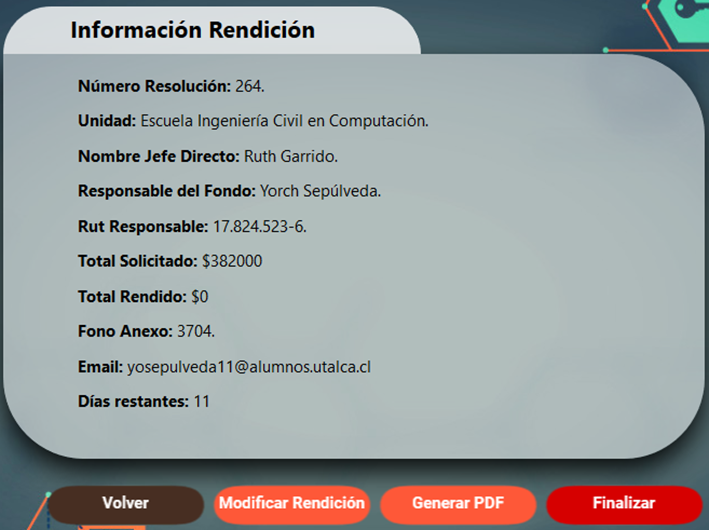
\includegraphics[width= \textwidth]{Imagenes/Rendicion.png}
    \caption{\label{fig: Rendicion}Vista que muestra los datos principales de una rendición o solicitud de reembolso.}
\end{figure}


    \subparagraph{\emph{Documento: }} Sección en donde se ingresan los datos de una boleta y/o factura, que corresponden al número del documento, la categoría en que incurrieron los gatos, la fecha de compra de los productos, el monto, una pequeña descripción de los gastos y el proveedor, entre otros (vea \textbf{Figura \ref{fig: AgregarBoletas}}).

    \begin{figure}[h]
        \centering
        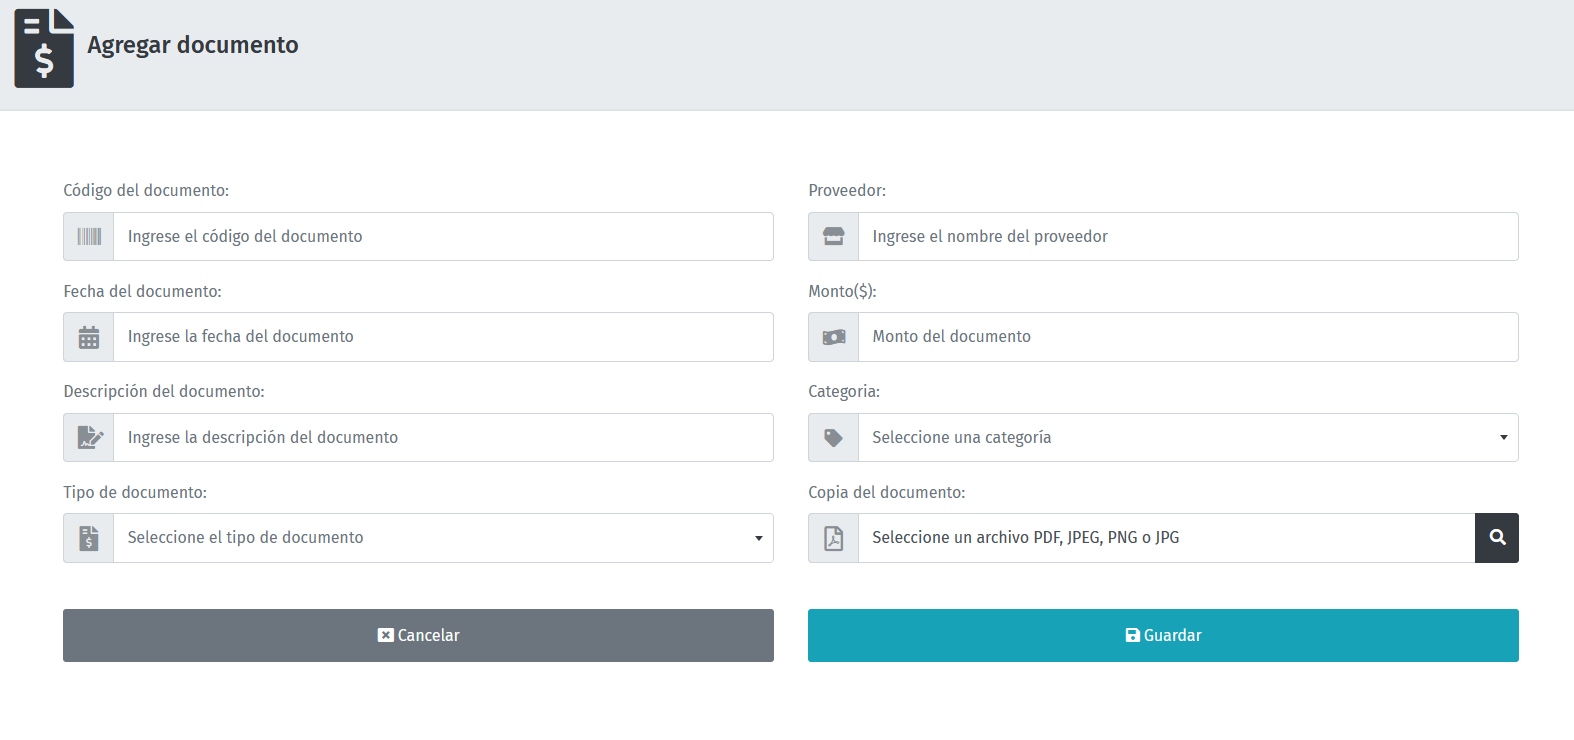
\includegraphics[width= \textwidth]{Imagenes/AgregarBoletas.PNG}
        \caption{\label{fig: AgregarBoletas}Vista que obtiene los datos de una boleta o factura.}
    \end{figure}




